 \documentclass[11pt]{article}

\usepackage{latexsym}
\usepackage{amssymb}
\usepackage{amsthm}
\usepackage{amscd}
\usepackage{amsmath}
\usepackage{tikz}
\usepackage[margin=1in]{geometry}
\usetikzlibrary{positioning}


\newtheorem{theorem}{Theorem}[section]
\newtheorem{fact}[theorem]{Fact}
\newtheorem{question}[theorem]{Question}
\newtheorem{claim}[theorem]{Claim}
\newtheorem{lemma}[theorem]{Lemma}
\newtheorem{definition}[theorem]{Definition}
\newtheorem{proposition}[theorem]{Proposition}
\newtheorem{corollary}[theorem]{Corollary}
\newtheorem{conjecture}[theorem]{Conjecture}

\theoremstyle{definition}
\newtheorem*{example}{Example}
\newtheorem*{remark}{Remark}
\newtheorem*{remarks}{Remarks}

\numberwithin{equation}{section}

\newcommand{\ZZ}{\mathbb{Z}}




\newcommand{\rook}{\hspace{-.1cm}\amalg\hspace{-.15cm}\bar{}}
\newcommand{\scscs}{\scriptscriptstyle} 
\newcommand{\scs}{\scriptstyle}




\begin{document}

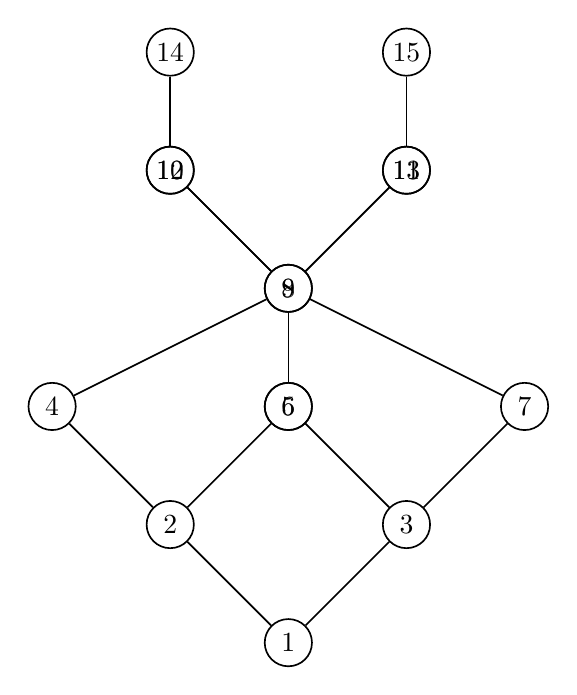
\begin{tikzpicture}[node distance=1.5cm and 1.5cm, on grid, semithick,
    state/.style={circle, draw, minimum size=0.6cm, inner sep=0pt}]

    % Nodes
    \node[state] (a) {1};
    \node[state] (b) [above left=of a] {2};
    \node[state] (c) [above right=of a] {3};
    \node[state] (d) [above left=of b] {4};
    \node[state] (e) [above right=of b] {5};
    \node[state] (f) [above left=of c] {6};
    \node[state] (g) [above right=of c] {7};
    \node[state] (h) [above=of e] {8};
    \node[state] (i) [above=of f] {9};
    \node[state] (j) [above left=of h] {10};
    \node[state] (k) [above right=of h] {11};
    \node[state] (l) [above left=of i] {12};
    \node[state] (m) [above right=of i] {13};
    \node[state] (n) [above=of j] {14};
    \node[state] (o) [above=of k] {15};

    % Edges (Lines)
    \draw (a) -- (b);
    \draw (a) -- (c);
    \draw (b) -- (d);
    \draw (b) -- (e);
    \draw (c) -- (f);
    \draw (c) -- (g);
    \draw (d) -- (h);
    \draw (e) -- (h);
    \draw (f) -- (i);
    \draw (g) -- (i);
    \draw (h) -- (j);
    \draw (h) -- (k);
    \draw (i) -- (l);
    \draw (i) -- (m);
    \draw (j) -- (n);
    \draw (k) -- (o);
    \draw (l) -- (n);
    \draw (m) -- (o);
    
\end{tikzpicture}



\end{document}



